% id: 82-11
% book: 100발100중 3-2 기말 · 01 3-2 기말(원의 성질·통계·부록)
% section: 실전 문제 1회 · 서술형 문제
% figure: crop:fig-82-11.png
% answer: $15\mkern3mu \%$
% answer_source: 답지(빠른정답)
% variant_level: 0 (원본 전사)
% 이 파일은 build.mjs 가 items.json 에서 만든다. 고칠 때는 items.json 을 고친다.
\smash{\raisebox{1.5mm}{\dmkichul{100발100중 3-2 기말 82쪽 11번 · 출제유력}}}
\noindent\begin{minipage}[t]{0.58\linewidth}\vspace{0pt}\raggedright 그림은 정미네 반 학생 20명의 두 차례에 걸친 공 던지기 기록을 조사하여 나타낸 산점도이다. 이때 1차와 2차 기록이 모두 $40\mkern3mu \mathrm{m}$ 이상인 학생은 전체의 몇 \%인지 구하고, 그 과정을 서술하시오. \mbox{[5점]}\end{minipage}\hfill\begin{minipage}[t]{0.4\linewidth}\vspace{0pt}\centering 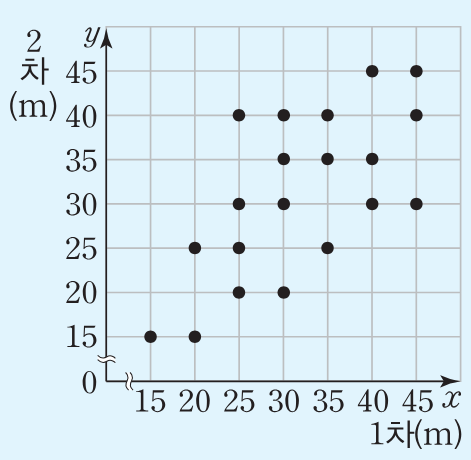
\includegraphics[width=112.9pt]{figures/fig-82-11.png}\end{minipage}\par
